\documentclass[@BEAMER_OPTIONS@]{beamer}
    @USE_PGFPAGES@

    \usetheme[alternativetitlepage=true,titleline=true]{Torino}
    \setbeamertemplate{navigation symbols}{}
    \setbeamertemplate{note page}[plain]

    \usepackage[utf8]{inputenc}
    \usepackage{graphicx}
    \usepackage{subfigure}
    \usepackage{xspace}
    \usepackage{adjustbox}
    \usepackage{tikz}
    \usepgflibrary{arrows}
    \usetikzlibrary{shadows,decorations.pathreplacing,patterns,shapes}
    \tikzstyle{every picture}=[semithick,>=stealth,remember picture]
    \usepackage{listings}
    \lstset{
        language=C++,
        basicstyle=\footnotesize\rmfamily,
        numbers=left,
        numberstyle=\tiny,
        aboveskip=-0.02\baselineskip,
        belowskip=-0.02\baselineskip,
        columns=flexible,
        extendedchars=false,
        showstringspaces=false
        }
    \newcommand{\code}[1]{\lstinline|#1|}
    \newcommand{\additive}{\hspace{1cm}\footnotesize(\emph{Additive expressions only})}
    \newcommand{\Cpp}{{C\nolinebreak[4]\hspace{-.05em}\raisebox{.4ex}{\tiny\bf ++}}\xspace}
    \newcommand{\ghribbon}{
        \begin{tikzpicture}[remember picture,overlay]
            \node[anchor=north east,yshift=4pt,xshift=4pt] at (current page.north east) {
                \href{https://github.com/ddemidov/vexcl}{
\includegraphics[width=2cm]{forkme}}
            };
        \end{tikzpicture}
    }

    \title{Converting generic \Cpp algorithms to OpenCL with VexCL library}

    \author{Denis Demidov}
    \institute{
        Supercomputer Center of Russian Academy of Sciences \\
        Kazan Federal University
    }
    \date{GPU-SMP 2013, Changchun, China}


\begin{document}

%----------------------------------------------------------------------------
\begin{frame}{}
    \titlepage
\end{frame}

\note{ }

%----------------------------------------------------------------------------
\begin{frame}{Modern GPGPU frameworks}
    \begin{columns}
        \begin{column}{0.45\textwidth}
            \begin{block}{CUDA}
                \begin{itemize}
                    \item Proprietary architecture by NVIDIA
                    \item Requires NVIDIA hardware
                    \item More mature, many libraries
                        \vspace{\baselineskip}
                    \item<2> \emph{Kernels are compiled to PTX together with
                        host program}
                \end{itemize}
            \end{block}
        \end{column}
        \begin{column}{0.45\textwidth}
            \begin{block}{OpenCL}
                \begin{itemize}
                    \item Open standard
                    \item Supports wide range of hardware
                    \item Code is much more verbose
                        \vspace{\baselineskip}
                    \item<2> \emph{Kernels are compiled at runtime, adding an
                        initialization overhead}
                \end{itemize}
            \end{block}
        \end{column}
    \end{columns}
    \vspace{\baselineskip}
    \begin{itemize}
        \item<2> The latter distinction is usually considered to be an OpenCL
            drawback.
        \item<2> But it also allows us to generate more efficient kernels at
            runtime!
    \end{itemize}
\end{frame}

\note[itemize]{
\item Today, major GPGPU programming frameworks are NVIDIA CUDA and OpenCL
\item ...
\item The latter distinction allows one to generate an OpenCL kernel tailored
    for the problem at hand.  And that is what I am going to talk about today.
}

%----------------------------------------------------------------------------
\begin{frame}{}
    \tableofcontents
\end{frame}

\note{
}

\section{VexCL overview}

%----------------------------------------------------------------------------
\begin{frame}{VexCL~--- a vector expression template library for OpenCL}
    \ghribbon
    \begin{itemize}
        \item \href{https://github.com/ddemidov/vexcl}{https://github.com/ddemidov/vexcl}
            \vspace{\baselineskip}
        \item Created for ease of \Cpp based OpenCL developement.
        \item The source code is publicly available under MIT license.
        \item \emph{This is not a} \Cpp \emph{bindings library!}
    \end{itemize}
\end{frame}

\note[itemize]{
\item VexCL is a vector expression template library for OpenCL. It uses
    template metaprogramming techniques (in particular, expression templates)
    to provide an intuitive notation for vector and matrix operations.
\item The source code of the library is available on GitHub. It is distributed
    under MIT license, so you are basically free to do whatever you want with
    the library.
\item I would like to note that this is not another \Cpp bindings library. VexCL
    is designed to work with standard \Cpp bindings for OpenCL that are provided
    by the Khronos group.
}

%----------------------------------------------------------------------------
\begin{frame}[fragile]{Hello VexCL: vector sum}
    \begin{exampleblock}{Get all available GPUs:}
        \begin{lstlisting}
vex::Context ctx( vex::Filter::Type(CL_DEVICE_TYPE_GPU) );
if ( !ctx ) throw std::runtime_error("GPUs not found");
        \end{lstlisting}
    \end{exampleblock}
    \begin{exampleblock}{Prepare input data, transfer it to device:}
        \begin{lstlisting}[firstnumber=last]
std::vector<float> a(N, 1), b(N, 2), c(N);
vex::vector<float> A(ctx, a);
vex::vector<float> B(ctx, b);
vex::vector<float> C(ctx, N);
        \end{lstlisting}
    \end{exampleblock}
    \begin{exampleblock}{Launch kernel, get result back to host:}
        \begin{lstlisting}[firstnumber=last]
C = A + B;
vex::copy(C, c);
std::cout << c[42] << std::endl;
        \end{lstlisting}
    \end{exampleblock}
\end{frame}

\note[itemize]{
\item Here is the simplest example of using vexcl: addition of two vectors on a
    gpu card.
\item First, we initialize VexCL context. We provide a device filter to the
    context constructor and get all compute devices that satisfy the filter.
    Here we filter by type and get all available GPUs.
\item Next, we allocate device vectors and transfer input data to devices.
\item Finally, we sum the input vectors in line 7. This simple expression leads
    to automatic generation and launch of OpenCL kernel.  Then we copy the
    results back to host and see what we got.
}

%----------------------------------------------------------------------------
\begin{frame}[fragile]{Memory and work splitting}
    \begin{exampleblock}{}
        \begin{onlyenv}<1|handout:0>
        \begin{lstlisting}[escapechar=!]
vex::Context ctx( !\color{chameleon4}{vex::Filter::Name("Tesla")}! );
        \end{lstlisting}
        \end{onlyenv}
        \begin{onlyenv}<2|handout:0>
        \begin{lstlisting}[escapechar=!]
vex::Context ctx( !\color{chameleon4}{vex::Filter::Type(CL\_DEVICE\_TYPE\_GPU)}! );
        \end{lstlisting}
        \end{onlyenv}
        \begin{onlyenv}<3>
        \begin{lstlisting}[escapechar=!]
vex::Context ctx( !\color{chameleon4}{vex::Filter::DoublePrecision}! );
        \end{lstlisting}
        \end{onlyenv}
        \begin{lstlisting}[firstnumber=last]

vex::vector<float> A(ctx, N); A = 1;
vex::vector<float> B(ctx, N); B = 2;
vex::vector<float> C(ctx, N);

C = A + B;
        \end{lstlisting}
    \end{exampleblock}
    \begin{figure}
        \begin{tikzpicture}
            \draw (0,3.0) rectangle +(8,0.1);
            \draw (0,3.0) grid[step=0.1] +(8,0.1);
            \draw (-0.3,3.1) node{A};

            \draw (0,2.5) rectangle +(8,0.1);
            \draw (0,2.5) grid[step=0.1] +(8,0.1);
            \draw (-0.3,2.6) node{B};

            \draw (0,2.0) rectangle +(8,0.1);
            \draw (0,2.0) grid[step=0.1] +(8,0.1);
            \draw (-0.3,2.1) node[anchor=center]{C};

            \uncover<1-3> {
            \draw (1,0.5) node{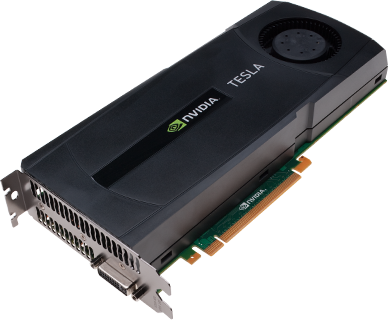
\includegraphics[width=0.2\textwidth]{tesla.png}};
            }

            \uncover<2-3> {
            \draw (4,0.5) node{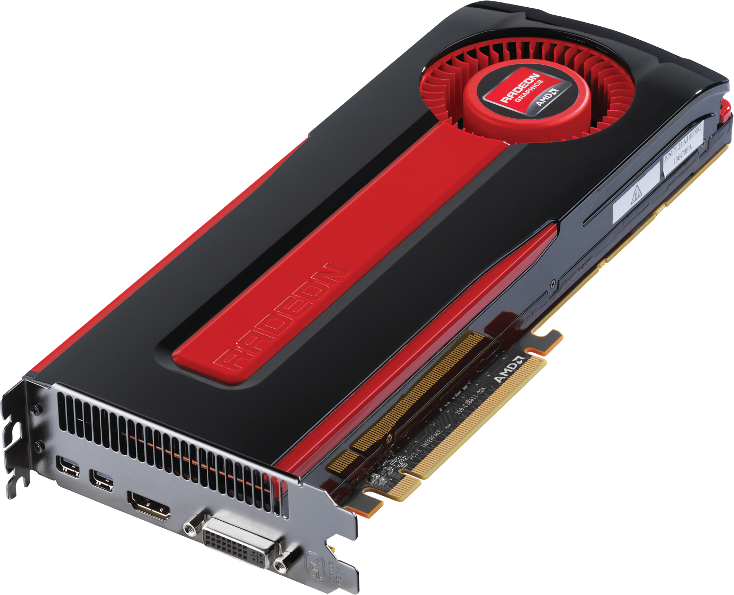
\includegraphics[width=0.2\textwidth]{radeon.png}};
            }

            \uncover<3> {
            \draw (7.5,0.5) node{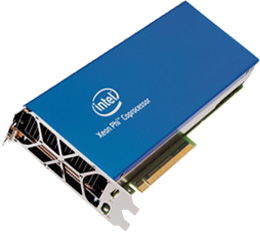
\includegraphics[width=0.16\textwidth]{intel.png}};
            }

            \uncover<1|handout:0> {
            \draw[->,chameleon3,style=dashed] (0,3.2) -- (0,1.8)
                .. controls +(east:0.5) and +(north west:0.5) ..
                (1.4,1.5);
            \draw[->,chameleon3,style=dashed] (8,3.2) -- (8,1.8)
                .. controls +(west:0.5) and +(north east:0.5) ..
                (1.6,1.5);
            }

            \uncover<2|handout:0> {
            \draw[->,chameleon3,style=dashed] (0,3.2) -- (0,1.8)
                .. controls +(east:0.5) and +(north west:0.5) ..
                (1.4,1.5);
            \draw[->,chameleon3,style=dashed] (4,3.2) -- (4,1.8)
                .. controls +(west:0.5) and +(north east:0.5) ..
                (1.6,1.5);

            \draw[->,chameleon3,style=dashed] (4,3.2) -- (4,1.8)
                .. controls +(east:0.1) and +(north west:0.2) ..
                (4.4,1.5);
            \draw[->,chameleon3,style=dashed] (8,3.2) -- (8,1.8)
                .. controls +(west:0.5) and +(north east:0.5) ..
                (4.6,1.5);
            }

            \uncover<3> {
            \draw[->,chameleon3,style=dashed] (0,3.2) -- (0,1.8)
                .. controls +(east:0.5) and +(north west:0.5) ..
                (1.4,1.5);
            \draw[->,chameleon3,style=dashed] (3.5,3.2) -- (3.5,1.8)
                .. controls +(west:0.5) and +(north east:0.5) ..
                (1.6,1.5);

            \draw[->,chameleon3,style=dashed] (3.5,3.2) -- (3.5,1.8)
                .. controls +(east:0.5) and +(north west:0.2) ..
                (4.4,1.5);
            \draw[->,chameleon3,style=dashed] (7,3.2) -- (7,1.8)
                .. controls +(west:0.5) and +(north east:0.5) ..
                (4.6,1.5);

            \draw[->,chameleon3,style=dashed] (7,3.2) -- (7,1.8) -- (7.4,1.5);
            \draw[->,chameleon3,style=dashed] (8,3.2) -- (8,1.8) -- (7.6,1.5);
            }
        \end{tikzpicture}
    \end{figure}
\end{frame}

\note[itemize]{
\item The memory and the workload is split between all devices in VexCL
    context. The share that each device gets is by default proportional to the
    device's bandwidth.
    \begin{enumerate}
        \item For example, if we only have the Tesla card in our context, then
            it will hold the complete memory for all of our vectors.
        \item If we use both of the available GPUs, then the vectors will be
            split between the devices. This split is by default proportional to
            the GPU bandwidth and is guaranteed to be consistent for vectors of
            the same size. This consistency allows VexCL to run computations
            independently on all devices in context.
        \item If we add the CPU to the context, it will get smaller share of
            the data and arithmetic operations.
    \end{enumerate}
}

%----------------------------------------------------------------------------
\begin{frame}[fragile]{What vector expressions are supported?}
    \begin{itemize}
        \item All vectors in an expression have to be \emph{compatible}:
            \begin{itemize}
                \item Have same size
                \item Located on same devices
            \end{itemize}
        \item What may be used:
            \begin{columns}
                \begin{column}{0.42\textwidth}
                    \begin{itemize}
                        \item Vectors and scalars
                        \item Arithmetic, logical operators
                        \item Built-in OpenCL functions
                        \item User-defined functions
                        \item Random number generators
                    \end{itemize}
                \end{column}
                \begin{column}{0.4\textwidth}
                    \begin{itemize}
                        \item Slicing and permutations
                        \item Reduction (sum, min, max)
                        \item Stencil operations
                        \item Sparse matrix~-- vector products
                        \item Fast Fourier Transform
                    \end{itemize}
                \end{column}
            \end{columns}
    \end{itemize}
    \begin{exampleblock}{}
        \begin{lstlisting}
vex::vector<double> x(ctx, n), y(ctx, n);

x = (2 * M_PI / n) * vex::element_index();
y = pow(sin(x), 2.0) + pow(cos(x), 2.0);
        \end{lstlisting}
    \end{exampleblock}
\end{frame}

\note[itemize]{
\item So, what kind of expressions can you use in VexCL?
\item First, any vectors used in an expression have to be compatible.
\item If this requirement is satisfied, then expressions may combine
    vectors and scalars with almost any binary operators. OpenCL math functions
    and user-defined functions are also available.
}

%----------------------------------------------------------------------------
\begin{frame}[fragile]{Each vector expression results in a single OpenCL kernel}
    \begin{columns}
        \begin{column}{0.38\textwidth}
            \begin{exampleblock}{The expression}
                \begin{lstlisting}
x = 2 * y - sin(z);
                \end{lstlisting}
            \end{exampleblock}
        \end{column}
        \begin{column}{0.55\textwidth}
            \begin{itemize}
                \item Boost.Proto is used as an expression template engine.
                \item Define \code{VEXCL_SHOW_KERNELS} to see the generated code.
            \end{itemize}
        \end{column}
    \end{columns}
    \begin{exampleblock}{\ldots results in this kernel:}
        \begin{lstlisting}
kernel void vexcl_vector_kernel(
    ulong n,
    global double * prm_1_1,
    int prm_1_2,
    global double * prm_1_3,
    global double * prm_1_4
)
{
    for(size_t idx = get_global_id(0); idx < n; idx += get_global_size(0)) {
        prm_1_1[idx] = ( ( prm_1_2 * prm_1_3[idx] ) - sin( prm_1_4[idx] ) );
    }
}
        \end{lstlisting}
    \end{exampleblock}
    \begin{tikzpicture}[overlay,scale=0.6]
        \draw (16,8) node(sub)[draw,fill=white,ellipse,drop shadow]{$-$};

        \draw (sub) +(-2.00,-1) node(mul)[draw,fill=white,drop shadow,ellipse]{$*$};
        \draw (sub) +( 2.00,-1) node(sin)[draw,fill=white,drop shadow,ellipse]{sin};
        \draw (mul) +(-2.00,-1) node(two)[draw,fill=white,drop shadow,minimum size=0.5cm]{2};
        \draw (mul) +( 1.50,-1) node(y)  [draw,fill=white,drop shadow,minimum size=0.5cm]{y};
        \draw (sin) +( 1.75,-1) node(z)  [draw,fill=white,drop shadow,minimum size=0.5cm]{z};

        \draw (sub) -- (mul);
        \draw (sub) -- (sin);
        \draw (mul) -- (two);
        \draw (mul) -- (y);
        \draw (sin) -- (z);
    \end{tikzpicture}
\end{frame}

\note[itemize]{
\item Boost.Proto is used as an expression template engine.
\item Expression tree terminals become kernel parameters, and the expression
    string is formed from the information encoded in the expression tree.
\item If you are curious, you can define \code{VEXCL_SHOW_KERNELS} macro before
    vexcl include pragma. This will show sources for every generated kernel on
    standard output.
}

%----------------------------------------------------------------------------
\section{Model problem}

\begin{frame}{}
    \tableofcontents[currentsection]
\end{frame}

\note{
}

%----------------------------------------------------------------------------
\begin{frame}[fragile]{Parameter study for Lorenz attractor system}
    \begin{columns}
        \begin{column}{0.6\textwidth}
            \begin{block}{Lorenz attractor system}
                \vspace{-1\baselineskip}
                \begin{align*}
                    \dot{x} &= -\sigma \left( x - y \right), \\
                    \dot{y} &= R x - y - xz, \\
                    \dot{z} &= -bz + xy.
                    \label{eq:lorenz}
                \end{align*}
            \end{block}
            \begin{itemize}
                \item Let's solve large number of Lorenz systems, each
                    for a different value of $R$.
                \item Let's use VexCL and Boost.odeint for that.
            \end{itemize}
        \end{column}
        \begin{column}{0.4\textwidth}
            \begin{figure}
                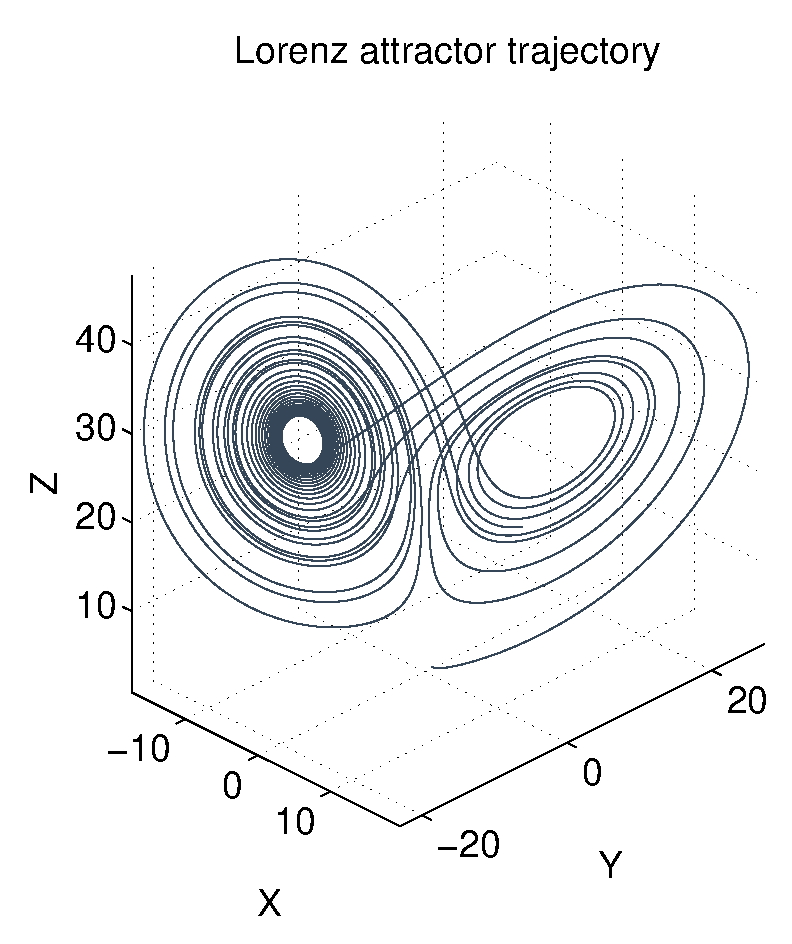
\includegraphics[width=\textwidth]{lorenz}
            \end{figure}
        \end{column}
    \end{columns}
\end{frame}

\note[itemize]{
\item As an example, lets solve a Lorenz attractor system of ordinary
    differential equations.
\item Lorenz attractor is a particle that moves according to these governing
    equations. The plot on the right shows an example of particle trajectory in
    time.
\item We will solve large number of these Lorenz systems at once.  Each of the
    systems will have its own value for parameter R. That's why this is called
    a parameter study.
}

%----------------------------------------------------------------------------
\begin{frame}{Using Boost.odeint}
    \begin{block}{ODE in general:}
        \begin{equation*}
            \frac{\mbox{d} x}{\mbox{d} t } = \dot{x} = f(x , t),
            \quad \quad x(0) = x_0.
        \end{equation*}
    \end{block}

    \vspace{\baselineskip}

    \begin{description}[\;]
        \item[Using Boost.odeint:] \quad
        \begin{enumerate}
            \item Define state type (what is $x$?)
            \item Provide system function (define $f$)
            \item Choose integration method
            \item Integrate over time
        \end{enumerate}
    \end{description}
\end{frame}

\note[itemize]{
\item Here is a general form of an ODE.
\item In order to use Boost.odeint, one has to...
}

\section{Naive implementation}

%----------------------------------------------------------------------------
\begin{frame}[fragile]{Naive implementation}
    \begin{exampleblock}{1. State type}
        \begin{lstlisting}
typedef vex::multivector<double, 3> state_type;
        \end{lstlisting}
    \end{exampleblock}

    \begin{exampleblock}{2. System functor}
        \begin{lstlisting}[firstnumber=last]
struct lorenz_system {
    const vex::vector<double> &R;
    lorenz_system(const vex::vector<double> &R ) : R(R) { }

    void operator()(const state_type &x, state_type &dxdt, double t) {
        dxdt = std::tie( sigma * ( x(1) - x(0) ),
                         R * x(0) - x(1) - x(0) * x(2),
                         x(0) * x(1) - b * x(2)  );
    }
};
        \end{lstlisting}
    \end{exampleblock}
\end{frame}

\note[itemize]{
\item We will hold current state of the system (or set of attractor
    coordinates) in a multivector with 3 components.
\item Here is the definition of the lorenz system functor: It computes the time
    derivative from current state and time (which is not used here).
\item VexCL make the definition of the functor very simple and intuitive: we
    assign a tuple of vector expressions to the multivector that represents
    time derivative.
}

%----------------------------------------------------------------------------
\begin{frame}[fragile]{Naive implementation}
    \begin{exampleblock}{3. Stepper (4th order Runge-Kutta)}
        \begin{lstlisting}[firstnumber=last]
odeint::runge_kutta4<
        state_type /*state*/,      double /*value*/,
        state_type /*derivative*/, double /*time*/,
        odeint::vector_space_algebra, odeint::default_operations
        > stepper;
        \end{lstlisting}
    \end{exampleblock}
    \begin{exampleblock}{4. Integration}
        \begin{lstlisting}[firstnumber=last]
vex::multivector<double,3> X(ctx, n);
vex::vector<double> R(ctx, n);

X = 10;
R = Rmin + vex::element_index() * ((Rmax - Rmin) / (n - 1));

odeint::integrate_const(stepper, lorenz_system(R), X, 0.0, t_max, dt);
        \end{lstlisting}
    \end{exampleblock}
\end{frame}

\note[itemize]{
\item Next, we create the stepper object and run the integration routine. Here
    we use classic 4th order Runge-Kutta method.
\item And that's it! This was really easy.
\item And, as you will see from the next slide, it was an order of magnitude
    faster than a multithreaded CPU variant.
}

%----------------------------------------------------------------------------
\begin{frame}[fragile]{Performance of naive implementation\footnote{
            \emph{Programming CUDA and OpenCL: A Case Study Using Modern C++
            Libraries}.\\
            \hspace{3em}Denis Demidov, Karsten Ahnert, Karl Rupp, Peter
            Gottschling. \href{http://arxiv.org/abs/1212.6326}{arXiv:1212.6326}
    }}
    \begin{figure}
        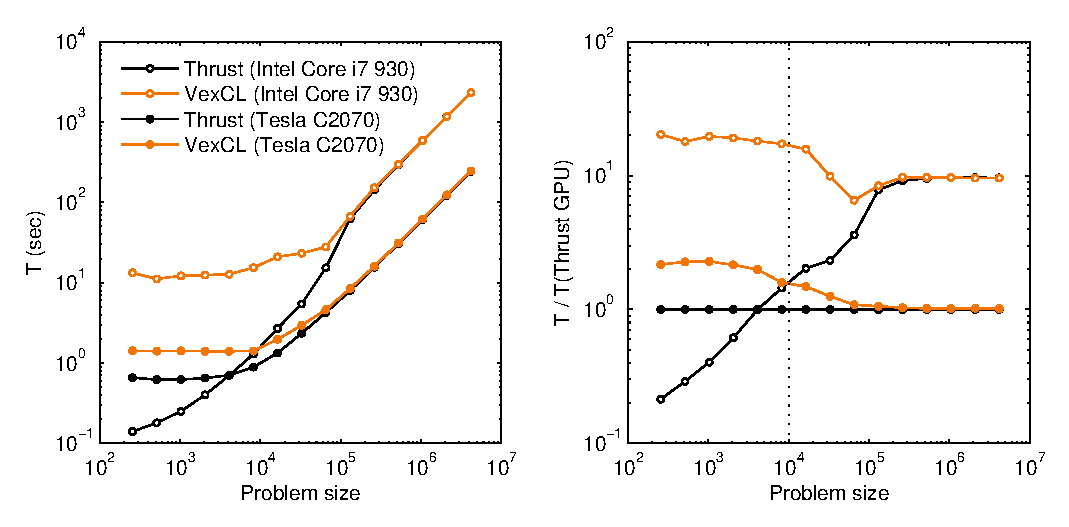
\includegraphics[width=0.8\textwidth]{perfnaive}
    \end{figure}
    \vspace{-1\baselineskip}
    \begin{itemize}
        \item GPU-based solution is 10 times faster!
            \uncover<2->{\alert{But,}}
            \begin{itemize}
                \item<2|alert@2> Runge-Kutta method uses 4 temporary state
                    variables (here stored on GPU).
                \item<2|alert@2> Single Runge-Kutta step results in several
                    kernel launches.
            \end{itemize}
    \end{itemize}
\end{frame}

\note[itemize]{
\item Here is performance of the naive implementation. I have also plotted
    results for CUDA-based Thrust library for comparison.
\item On the left plot you see absolute running times for problems of different
    sizes. Right plot depicts times relative to Thrust solution on GPU.
\item Black lines correspond to Thrust, orange lines -- to VexCL.
\item Filled markers are GPU times, and empty markers are CPU times.
\item You see that both CUDA and OpenCL have high overhead for small problems,
    so CPU-based Thrust solution is the fastest there.
\item But we are interested in results for larger problems. Here VexCL variant
    shows performance equal to Thrust's. The solution on a GPU is ten times
    faster than on a CPU for both libraries.
}

%----------------------------------------------------------------------------
\begin{frame}[fragile]{What if we did this manually?}
    \begin{columns}
        \begin{column}{0.45\textwidth}
            \begin{itemize}
                \item Create monolithic kernel for a single step of Runge-Kutta
                    method.
                \item Launch the kernel in a loop.
                    \vspace{\baselineskip}
                \item This is another 10x faster!
                    \uncover<2->{\alert{But,}}
                    \begin{itemize}
                        \item<2|alert@2> We lost odeint's generality.
                    \end{itemize}
            \end{itemize}
        \end{column} \quad \quad
        \begin{column}{0.5\textwidth}
            \begin{exampleblock}{}
                \begin{adjustbox}{width=0.95\textwidth,height=0.95\textheight,keepaspectratio}
                    \begin{lstlisting}
double3 lorenz_system(double r, double sigma, double b, double3 s) {
    return (double3)( sigma * (s.y - s.x),
                       r * s.x - s.y - s.x * s.z,
                       s.x * s.y - b * s.z);
}
kernel void lorenz_ensemble(
    ulong  n, double dt, double sigma, double b,
    const global double *R,
    global double *X,
    global double *Y,
    global double *Z
    )
{
    for(size_t i = get_global_id(0); i < n; i += get_global_size(0)) {
        double  r = R[i];
        double3 s = (double3)(X[i], Y[i], Z[i]);
        double3 k1, k2, k3, k4;

        k1 = dt * lorenz_system(r, sigma, b, s);
        k2 = dt * lorenz_system(r, sigma, b, s + 0.5 * k1);
        k3 = dt * lorenz_system(r, sigma, b, s + 0.5 * k2);
        k4 = dt * lorenz_system(r, sigma, b, s + k3);

        s += (k1 + 2 * k2 + 2 * k3 + k4) / 6;

        X[i] = s.x; Y[i] = s.y; Z[i] = s.z;
    }
}
                    \end{lstlisting}
                \end{adjustbox}
            \end{exampleblock}
        \end{column}
    \end{columns}
\end{frame}

\note[itemize]{
\item So, what if we did this manually?
\item We would create a single kernel that would do complete Runge-Kutta
    integration step. By the way, here is the kernel that does just that. It's
    very nice-looking kernel in fact.
\item If we run this kernel in a loop, it would give us our solution. And it
    would be ten times faster than our previous variant. So a hundred times
    faster than a CPU! That's an acceleration!
\item But, odeint has 20 different steppers. We don't want to reimplement all
    of those. Let Karsten here do the job, right?
}

\section{Kernel generator}

%----------------------------------------------------------------------------
\begin{frame}{}
    \tableofcontents[currentsection]
\end{frame}

\note{}

%----------------------------------------------------------------------------
\begin{frame}[fragile]{Convert Boost.odeint stepper to OpenCL kernel}
    \begin{itemize}
        \item VexCL provides \code{vex::generator::symbolic<T>} type.
        \item An instance of the type dumps any arithmetic operations to output
            stream:
    \end{itemize}
    \begin{exampleblock}{}
        \begin{lstlisting}
vex::generator::symbolic<double> x = 6, y = 7;
x = sin(x * y);
        \end{lstlisting}
    \end{exampleblock}
    \begin{small}
        \begin{verbatim}
double var1 = 6;
double var2 = 7;
var1 = sin( ( var1 * var2 ) );
        \end{verbatim}
    \end{small}
\end{frame}

\note[itemize]{
\item VexCL allows to achieve same effect without manual coding.
\item The idea is very simple:
    \begin{itemize}
        \item An algorithm (any algorithm) is just a sequence of arithmetic
            expressions.
        \item VexCL symbolic types allow to record such expressions.
    \end{itemize}
}

%----------------------------------------------------------------------------
\begin{frame}[fragile]{Record operations performed by Boost.odeint stepper}
    \begin{exampleblock}{1. State type}
        \begin{lstlisting}
typedef vex::generator::symbolic< double > sym_vector;
typedef std::array<sym_vector, 3> sym_state;
        \end{lstlisting}
    \end{exampleblock}

    \begin{exampleblock}{2. System functor}
        \begin{lstlisting}[firstnumber=last]
struct lorenz_system {
    const sym_vector &R;
    lorenz_system(const sym_vector &R) : R(R) {}

    void operator()(const sym_state &x, sym_state &dxdt, double t) const {
        dxdt[0] = sigma * (x[1] - x[0]);
        dxdt[1] = R * x[0] - x[1] - x[0] * x[2];
        dxdt[2] = x[0] * x[1] - b * x[2];
    }
};
        \end{lstlisting}
    \end{exampleblock}
\end{frame}

\note[itemize]{
\item Let's record the sequence of expressions that, for example, Runge-Kutta
    method does, and let's build an OpenCL kernel from this sequence.
\item We replace the state type with array of three symbolic variables. We also
    slightly modify our system functor.
}

%----------------------------------------------------------------------------
\begin{frame}[fragile]{Record operations performed by Boost.odeint stepper}
    \begin{exampleblock}{3. Stepper}
        \begin{lstlisting}[firstnumber=last]
odeint::runge_kutta4<
        sym_state /*state*/,      double /*value*/,
        sym_state /*derivative*/, double /*time*/,
        odeint::range_algebra, odeint::default_operations
        > stepper;
        \end{lstlisting}
    \end{exampleblock}

    \begin{exampleblock}{4. Record one step of Runge-Kutta method}
        \begin{lstlisting}[firstnumber=last]
std::ostringstream lorenz_body;
vex::generator::set_recorder(lorenz_body);

sym_state sym_S = {{ sym_vector(sym_vector::VectorParameter),
                      sym_vector(sym_vector::VectorParameter),
                      sym_vector(sym_vector::VectorParameter) }};
sym_vector sym_R(sym_vector::VectorParameter, sym_vector::Const);

lorenz_system sys(sym_R);
stepper.do_step(std::ref(sys), sym_S, 0, dt);
        \end{lstlisting}
    \end{exampleblock}
\end{frame}

\note[itemize]{
\item We also alter the stepper type accordingly.
\item Next we create the string stream and register it as the expression
    recorder.
\item Finally, we create symbolic variables that would correspond to generated
    kernel parameters, and run single integration step.
\item Now lorenz\_body holds the recorded expression sequence that we
    need.
}

%----------------------------------------------------------------------------
\begin{frame}[fragile]{Generate OpenCL kernel with the recorded sequence}
    \begin{exampleblock}{5. Generate and use OpenCL kernel}
        \begin{lstlisting}[firstnumber=last]
auto lorenz_kernel = vex::generator::build_kernel(ctx, "lorenz", lorenz_body.str(),
        sym_S[0], sym_S[1], sym_S[2], sym_R);

vex::vector<double> X(ctx, n), Y(ctx, n), Z(ctx, n), R(ctx, n);

X = Y = Z = 10;
R = Rmin + (Rmax - Rmin) * vex::element_index() / (n - 1);

for(double t = 0; t < t_max; t += dt) lorenz_kernel(X, Y, Z, R);
        \end{lstlisting}
    \end{exampleblock}
\end{frame}

\note[itemize]{
\item We generate the OpenCL kernel named "lorenz" with the information from
    \code{lorenz_body}. We also supply the symbolic vectors that participated
    in our algorithm. Those will become kernel parameters.
\item Next we create our device vectors, and run the integration loop with the
    generated kernel.
\item And this could be done for any of 20 odeint steppers or for almost any
    other generic algorithm!
}

%----------------------------------------------------------------------------
\begin{frame}{The restrictions}
    \begin{itemize}
        \item Algorithms have to be embarrassingly parallel.
        \item Only linear flow is allowed (no conditionals or data-dependent
            loops).
        \item Some precision may be lost when converting constants to strings.
        \item Probably some other corner cases\ldots
    \end{itemize}
\end{frame}

\note[itemize]{
\item Of course, there are some restrictions.
}

%----------------------------------------------------------------------------
\begin{frame}[fragile]{Performance of the generated kernel}
    \begin{figure}
        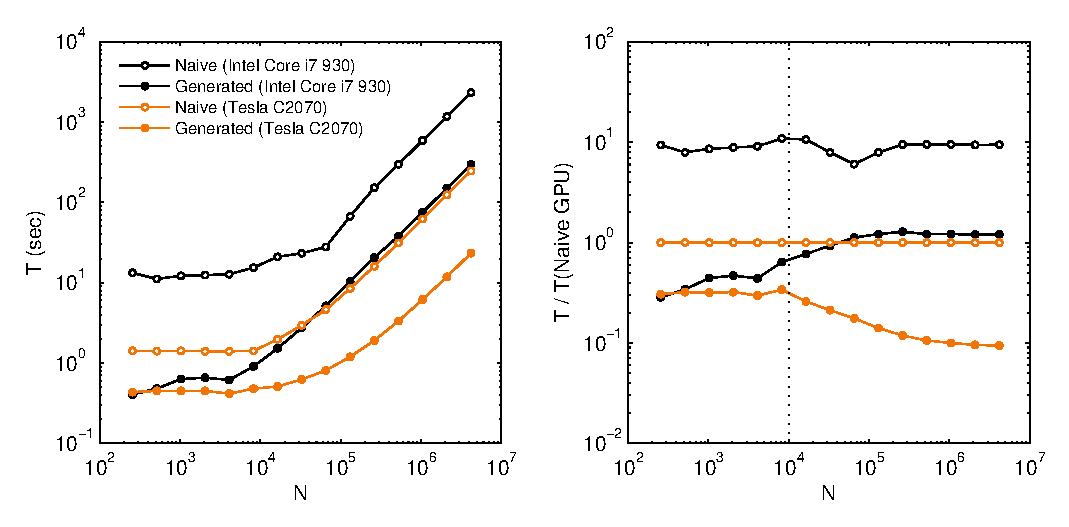
\includegraphics[width=0.9\textwidth]{perfgen}
    \end{figure}
\end{frame}

\note[itemize]{
\item But, as you can see from this slide, the technique allows to achive same
    acceleration we got from manually coded kernel (Both for CPU and GPU).
}

\section{Function generator}

%----------------------------------------------------------------------------
\begin{frame}{}
    \tableofcontents[currentsection]
\end{frame}

\note{}

%----------------------------------------------------------------------------
\begin{frame}[fragile]{Function generator}
    \begin{itemize}
        \item Built on top of symbolic types
        \item Converts generic \Cpp functor to a VexCL function
    \end{itemize}

    \begin{exampleblock}{Simple example: compute square radius for 2D points}
        \begin{equation*}
            R^2 = X^2 + Y^2
        \end{equation*}
    \end{exampleblock}

    \begin{itemize}
        \item We want to define a VexCL function \code{sqr()} that may be used
            in vector expressions like these:
    \end{itemize}
    \begin{exampleblock}{}
        \begin{lstlisting}
R2 = sqr(X, Y);
R = sqrt(sqr(X, Y));
Z = sqr(sin(X), cos(Y));
        \end{lstlisting}
    \end{exampleblock}
\end{frame}

\note{ }

%----------------------------------------------------------------------------
\begin{frame}[fragile]{v1. Provide body for OpenCL function}
    \begin{exampleblock}{}
        \begin{lstlisting}
vex::vector<double> X(ctx, N), Y(ctx, N), R2(ctx, N);

VEX_FUNCTION(sqr, double(double, double), "return prm1 * prm1 + prm2 * prm2;");

R2 = sqr(X, Y);
        \end{lstlisting}
    \end{exampleblock}

    \begin{itemize}
        \item Easy enough (for simple functions)
        \item But needs separate code for host-side and OpenCL paths
    \end{itemize}
\end{frame}

\note[itemize]{
\item First, we can use VEX\_FUNCTION macro to define a VexCL function
\item Here, we provide the name of the function, its signature, and textual
    representation of its body.
\item Its not that complicated, but we would need to code a host-side path
    separately.
}

%----------------------------------------------------------------------------
\begin{frame}[fragile]{v2. Using Function generator and a generic functor}
    \begin{exampleblock}{1. Define generic functor}
        \begin{lstlisting}
struct square_radius {
    template <class T>
    T operator()(const T &x, const T &y) const {
        return x * x + y * y;
    }
};
        \end{lstlisting}
    \end{exampleblock}
    \begin{exampleblock}{2. Use it to generate a VexCL function}
        \begin{lstlisting}
using vex::generator::make_function;

auto sqr = make_function<double(double, double)>( square_radius() );

R2 = sqr(X, Y);
        \end{lstlisting}
    \end{exampleblock}

    \begin{itemize}
        \item Allows to reuse same functor for host-side and OpenCL paths
    \end{itemize}
\end{frame}

\note[itemize]{
\item We can solve this problem with help of function generator and a generic
    functor.
\item The functor may be used both for host-side code and for the generation of
    VexCL functions.
\item This works very simple: knowing the function signature, the function
    generator creates the required symbolic instances and passes them to the
    generic functor. This provides the generator with the textual
    representation for the function body.
}

%----------------------------------------------------------------------------
\begin{frame}[fragile]{v3. Using Function generator and a Boost.Phoenix lambda}
    \begin{itemize}
        \item Boost.Phoenix lambdas are generic functors in disguise
        \item Hence, the following is possible:
    \end{itemize}

    \begin{exampleblock}{}
        \begin{lstlisting}
using namespace boost::phoenix::arg_names;

auto sqr = make_function<double(double, double)>(arg1 * arg1 + arg2 * arg2);

R2 = sqr(X, Y);
        \end{lstlisting}
    \end{exampleblock}
\end{frame}

\note[itemize]{
\item Boost.Phoenix is a lambda library.
\item And it so happens that Phoenix lambdas are in fact generic functors.
}

\section{Summary}

%----------------------------------------------------------------------------
\begin{frame}{Summary}
    \ghribbon
    \begin{itemize}
        \item VexCL allows to write compact and readable code
            without sacrificing performance.
        \item Its code generator allows to convert generic \Cpp
            code to OpenCL at runtime:
            \begin{itemize}
                \item Reduces global memory I/O
                \item Reduces number of kernel launches
                \item Does not require change of existing code
                \item Facilitates code reuse
            \end{itemize}
            \vspace{\baselineskip}
            \vspace{\baselineskip}
        \item \href{https://github.com/ddemidov/vexcl}
            {https://github.com/ddemidov/vexcl}
    \end{itemize}
\end{frame}

\note{ }

\end{document}

% vim: et
